% ============================================================
% Screw Metrology Pipeline V2 — Technical Documentation
% XIS AI / Computer Vision Department — Assessment Submission
% ============================================================
\documentclass[12pt, a4paper, twoside]{report}

% ─── Packages ────────────────────────────────────────────────
\usepackage[utf8]{inputenc}
\usepackage[T1]{fontenc}
\usepackage{lmodern}
\usepackage[margin=2.5cm]{geometry}
\usepackage{graphicx}
\usepackage{amsmath, amssymb}
\usepackage{booktabs}
\usepackage{tabularx}
\usepackage{longtable}
\usepackage{xcolor}
\usepackage{hyperref}
\usepackage{listings}
\usepackage{fancyhdr}
\usepackage{enumitem}
\usepackage{float}
\usepackage{caption}
\usepackage{subcaption}
\usepackage{tikz}
\usepackage{pgfplots}
\pgfplotsset{compat=1.18}
\usepackage{tcolorbox}
\usepackage{titlesec}
\usepackage{pdfpages}
\usepackage{array}
\usepackage{multirow}
\usepackage{makecell}
\usepackage{setspace}

% ─── Colors ──────────────────────────────────────────────────
\definecolor{xisblue}{HTML}{1565C0}
\definecolor{xisdark}{HTML}{0D1117}
\definecolor{xisgray}{HTML}{6E7781}
\definecolor{codebg}{HTML}{F6F8FA}
\definecolor{codegreen}{HTML}{22863A}
\definecolor{codepurple}{HTML}{6F42C1}
\definecolor{codeblue}{HTML}{005CC5}
\definecolor{passfg}{HTML}{1B5E20}
\definecolor{passbg}{HTML}{E8F5E9}
\definecolor{warnfg}{HTML}{E65100}
\definecolor{warnbg}{HTML}{FFF3E0}

% ─── Hyperlink Setup ─────────────────────────────────────────
\hypersetup{
    colorlinks=true,
    linkcolor=xisblue,
    citecolor=xisblue,
    urlcolor=xisblue,
    pdftitle={Screw Metrology Pipeline V2 — Technical Documentation},
    pdfauthor={Aroon Kumar},
}

% ─── Code Listing Style ─────────────────────────────────────
\lstdefinestyle{pythonstyle}{
    backgroundcolor=\color{codebg},
    basicstyle=\ttfamily\footnotesize,
    keywordstyle=\color{codepurple}\bfseries,
    stringstyle=\color{codegreen},
    commentstyle=\color{xisgray}\itshape,
    numberstyle=\tiny\color{xisgray},
    breaklines=true,
    frame=single,
    rulecolor=\color{xisgray!30},
    numbers=left,
    numbersep=8pt,
    tabsize=4,
    showstringspaces=false,
    language=Python,
    morekeywords={self, True, False, None, as, import, from, return, def, class, with, yield},
}
\lstdefinestyle{bashstyle}{
    backgroundcolor=\color{xisdark},
    basicstyle=\ttfamily\footnotesize\color{white},
    breaklines=true,
    frame=single,
    rulecolor=\color{xisgray!50},
    numbers=none,
    tabsize=4,
    showstringspaces=false,
}
\lstset{style=pythonstyle}

% ─── Header/Footer ──────────────────────────────────────────
\pagestyle{fancy}
\fancyhf{}
\fancyhead[LE]{\small\textcolor{xisgray}{\leftmark}}
\fancyhead[RO]{\small\textcolor{xisgray}{\rightmark}}
\fancyfoot[C]{\small\textcolor{xisgray}{Page \thepage}}
\fancyfoot[LE,RO]{\small\textcolor{xisgray}{Screw Metrology Pipeline V2}}
\renewcommand{\headrulewidth}{0.4pt}
\renewcommand{\footrulewidth}{0.2pt}

% ─── tcolorbox environments ─────────────────────────────────
\newtcolorbox{notebox}{
    colback=blue!5!white,
    colframe=xisblue,
    title={\textbf{Note}},
    fonttitle=\bfseries\color{white},
    coltitle=white,
    arc=2mm,
    boxrule=0.5pt,
}

\newtcolorbox{importantbox}{
    colback=warnbg,
    colframe=warnfg,
    title={\textbf{Important}},
    fonttitle=\bfseries\color{white},
    coltitle=white,
    arc=2mm,
    boxrule=0.5pt,
}

\newtcolorbox{tipbox}{
    colback=passbg,
    colframe=passfg,
    title={\textbf{Tip}},
    fonttitle=\bfseries\color{white},
    coltitle=white,
    arc=2mm,
    boxrule=0.5pt,
}

% ─── Chapter formatting ─────────────────────────────────────
\titleformat{\chapter}[display]
    {\normalfont\Huge\bfseries\color{xisblue}}
    {\chaptertitlename\ \thechapter}{20pt}{\Huge}
\titlespacing*{\chapter}{0pt}{-20pt}{30pt}

% ─── Document Info ───────────────────────────────────────────
\title{
    \vspace{-2cm}
    \textcolor{xisblue}{\rule{\linewidth}{2pt}}\\[0.8cm]
    {\Huge\bfseries Screw Metrology Pipeline V2}\\[0.4cm]
    {\Large Technical Documentation}\\[0.3cm]
    {\large XIS AI / Computer Vision Department}\\[0.3cm]
    {\large Technical Assessment Submission}\\[0.5cm]
    \textcolor{xisblue}{\rule{\linewidth}{2pt}}
}
\author{
    \textbf{Aroon Kumar}\\[0.2cm]
    \texttt{github.com/AroonKumarr/Screw-Metrology-Pipeline-V2}
}
\date{\today}

% ============================================================
\begin{document}
\maketitle
\thispagestyle{empty}

% ─── Abstract ────────────────────────────────────────────────
\begin{abstract}
\noindent
This document presents the complete technical documentation for the \textbf{Screw Metrology Pipeline V2} --- an end-to-end computer vision system that segments hex-head machine screws from images and computes their real-world width (diameter) and height (length) in millimetres. The pipeline integrates three stages: (1)~intrinsic camera calibration using a checkerboard pattern to remove lens distortion, (2)~instance segmentation using Mask~R-CNN with a ResNet-50+FPN backbone fine-tuned on 51 custom-labelled images, and (3)~metric measurement using an ArUco fiducial marker as a physical scale reference. On the held-out test set, the model achieves mAP@0.5~=~1.000, mAP@0.5:0.95~=~0.775, and Mean~IoU~=~0.861. Measurement accuracy against physical calliper ground truth yields a width MAE of 0.019\,mm and length MAE of 0.067\,mm, both well within the target thresholds of $<5\%$ and $<2\%$ MPE respectively.
\end{abstract}

\tableofcontents
\listoffigures
\listoftables

% ============================================================
% CHAPTER 1: PROJECT OVERVIEW
% ============================================================
\chapter{Project Overview}
\label{ch:overview}

\section{What the System Does}
The Screw Metrology Pipeline V2 is an industrial-grade computer vision system designed to:
\begin{enumerate}
    \item \textbf{Correct optical distortion} from smartphone camera lenses using intrinsic camera calibration.
    \item \textbf{Segment individual screws} from complex backgrounds using deep learning instance segmentation.
    \item \textbf{Measure physical dimensions} (width in mm, height in mm) from pixel data using a known-size ArUco reference marker.
\end{enumerate}

\section{Key Capabilities}
\begin{itemize}
    \item \textbf{Instance-level segmentation:} Each screw receives its own binary mask, enabling independent measurement even when multiple screws are present.
    \item \textbf{Rotation-invariant measurement:} Uses \texttt{cv2.minAreaRect} (minimum area rotated bounding box) instead of axis-aligned boxes, so screws at any angle are measured correctly.
    \item \textbf{Sub-millimetre accuracy:} Width MAE = 0.019\,mm, Length MAE = 0.067\,mm.
    \item \textbf{EXIF-aware image loading:} Handles the smartphone EXIF rotation metadata bug that causes coordinate misalignment between annotations and raw pixel arrays.
    \item \textbf{End-to-end reproducibility:} Fixed random seed, version-pinned dependencies, single-command pipeline execution.
\end{itemize}

\section{Key Results Summary}
\begin{table}[H]
\centering
\caption{Model performance on held-out test set (10\% split, 4 images).}
\label{tab:key-results}
\begin{tabular}{lcc}
\toprule
\textbf{Metric} & \textbf{Score} & \textbf{Assessment} \\
\midrule
mAP@0.5                & 1.000   & \textcolor{passfg}{\textbf{Pass}} \\
mAP@0.5:0.95           & 0.775   & \textcolor{passfg}{\textbf{Pass}} \\
Mean IoU               & 0.861   & \textcolor{passfg}{\textbf{Pass}} \\
Precision              & 1.000   & \textcolor{passfg}{\textbf{Pass}} \\
Recall                 & 1.000   & \textcolor{passfg}{\textbf{Pass}} \\
F1-Score               & 1.000   & \textcolor{passfg}{\textbf{Pass}} \\
Width MAE              & 0.019\,mm & \textcolor{passfg}{\textbf{Pass}} \\
Length MAE             & 0.067\,mm & \textcolor{passfg}{\textbf{Pass}} \\
\bottomrule
\end{tabular}
\end{table}

\section{Measurement Target: Hex-Head Machine Screws}
The physical object chosen for this pipeline is a \textbf{hex-head machine screw} with approximate dimensions:
\begin{itemize}
    \item \textbf{Diameter (width):} $\sim 4.2$\,mm
    \item \textbf{Length (height):} $\sim 22.5$\,mm
\end{itemize}

\noindent\textbf{Justification for object choice:}
\begin{itemize}
    \item \textbf{Rigid geometry:} The cylindrical shaft and hexagonal head provide sharp, well-defined polygon boundaries ideal for instance segmentation.
    \item \textbf{Industrial relevance:} Screw dimensioning is a real-world quality control task in manufacturing.
    \item \textbf{Labelling ease:} High contrast between metallic screw surface and paper/desk backgrounds makes polygon annotation unambiguous.
    \item \textbf{Availability:} Ubiquitous hardware store item, easy to photograph in various setups.
\end{itemize}


% ============================================================
% CHAPTER 2: SETUP & INSTALLATION GUIDE
% ============================================================
\chapter{Setup \& Installation Guide}
\label{ch:setup}

\section{Prerequisites}
\begin{table}[H]
\centering
\caption{System requirements.}
\begin{tabular}{lll}
\toprule
\textbf{Component} & \textbf{Minimum} & \textbf{Recommended} \\
\midrule
Python       & 3.9+      & 3.11+ \\
CPU          & 4 cores   & 8+ cores \\
RAM          & 8\,GB     & 16+\,GB \\
GPU          & ---       & NVIDIA 6+\,GB VRAM \\
Storage      & 5\,GB     & 20+\,GB \\
OS           & macOS / Linux / Windows & Any \\
\bottomrule
\end{tabular}
\end{table}

\section{Step-by-Step Installation}

\subsection{Clone the Repository}
\begin{lstlisting}[style=bashstyle]
git clone https://github.com/AroonKumarr/Screw-Metrology-Pipeline-V2.git
cd Screw-Metrology-Pipeline-V2
\end{lstlisting}

\subsection{Create Virtual Environment}
\begin{lstlisting}[style=bashstyle]
python -m venv venv
source venv/bin/activate       # macOS / Linux
# venv\Scripts\activate        # Windows
\end{lstlisting}

\subsection{Install Dependencies}
\begin{lstlisting}[style=bashstyle]
pip install --upgrade pip
pip install -r requirements.txt
\end{lstlisting}

\subsection{PyTorch with CUDA (Optional, for GPU Training)}
\begin{lstlisting}[style=bashstyle]
# For CUDA 11.8
pip install torch torchvision --index-url https://download.pytorch.org/whl/cu118

# For CUDA 12.1
pip install torch torchvision --index-url https://download.pytorch.org/whl/cu121
\end{lstlisting}

\subsection{Verify Installation}
\begin{lstlisting}[style=pythonstyle]
import torch, torchvision, cv2, numpy as np
print(f"PyTorch:     {torch.__version__}")
print(f"TorchVision: {torchvision.__version__}")
print(f"OpenCV:      {cv2.__version__}")
print(f"NumPy:       {np.__version__}")
print(f"CUDA:        {torch.cuda.is_available()}")
\end{lstlisting}

\section{Python Dependencies}
The full dependency list (from \texttt{requirements.txt}):

\begin{table}[H]
\centering
\caption{Python package dependencies.}
\begin{tabular}{lll}
\toprule
\textbf{Category} & \textbf{Package} & \textbf{Version} \\
\midrule
Deep Learning   & \texttt{torch}                & $\geq$ 2.0.0 \\
                & \texttt{torchvision}          & $\geq$ 0.15.0 \\
\midrule
Computer Vision & \texttt{opencv-python}        & $\geq$ 4.8.0 \\
                & \texttt{opencv-contrib-python} & $\geq$ 4.8.0 \\
\midrule
Data Science    & \texttt{numpy}                & $\geq$ 1.24.0 \\
                & \texttt{pandas}               & $\geq$ 2.0.0 \\
                & \texttt{scipy}                & $\geq$ 1.10.0 \\
                & \texttt{scikit-learn}          & $\geq$ 1.3.0 \\
\midrule
Image Processing & \texttt{Pillow}              & $\geq$ 10.0.0 \\
                 & \texttt{albumentations}       & $\geq$ 1.3.0 \\
\midrule
COCO Tools      & \texttt{pycocotools}          & $\geq$ 2.0.7 \\
\midrule
Visualisation   & \texttt{matplotlib}           & $\geq$ 3.7.0 \\
                & \texttt{seaborn}              & $\geq$ 0.12.0 \\
\midrule
Utilities       & \texttt{tqdm}                 & $\geq$ 4.65.0 \\
                & \texttt{pyyaml}               & $\geq$ 6.0 \\
\midrule
Notebook        & \texttt{jupyter}              & $\geq$ 1.0.0 \\
                & \texttt{ipykernel}            & $\geq$ 6.0.0 \\
\bottomrule
\end{tabular}
\end{table}

\section{Running the Pipeline}

\subsection{Notebook (Recommended)}
\begin{lstlisting}[style=bashstyle]
jupyter notebook notebooks/screw_metrology_pipeline.ipynb
\end{lstlisting}

\subsection{CLI Commands}
\begin{lstlisting}[style=bashstyle]
# Camera Calibration
python main.py calibrate --images calibration/images/ --output calibration/output/

# Dataset Split (70/20/10)
python scripts/split_dataset.py

# Train Model
python main.py train --data-dir dataset/ \
  --train-ann dataset/annotations/train.json \
  --val-ann dataset/annotations/val.json --epochs 15

# Evaluate on Test Set
python main.py evaluate --model models/weights/best_model.pth \
  --test-dir dataset/train/images \
  --test-ann dataset/annotations/test.json

# Measure a Screw
python main.py measure --image my_screw.jpg \
  --model models/weights/best_model.pth \
  --calibration-dir calibration/output/ --marker-size 198.0
\end{lstlisting}


% ============================================================
% CHAPTER 3: SYSTEM / PIPELINE ARCHITECTURE
% ============================================================
\chapter{System / Pipeline Architecture}
\label{ch:architecture}

\section{End-to-End Data Flow}
The pipeline processes a raw smartphone photograph through four sequential stages, each resolving a specific spatial or optical ambiguity:

\begin{figure}[H]
\centering
\begin{tikzpicture}[
    node distance=1.4cm,
    block/.style={rectangle, draw=xisblue, fill=blue!5, text width=12cm, minimum height=1.2cm, align=center, rounded corners=3pt, font=\small},
    arrow/.style={->, thick, color=xisblue},
    label/.style={font=\footnotesize\itshape, color=xisgray}
]
\node[block] (raw) {\textbf{Stage 0: Raw Image Input}\\EXIF Transpose $\rightarrow$ Correct portrait orientation (3024$\times$4032\,px)};
\node[block, below=of raw] (undist) {\textbf{Stage 1: Lens Undistortion}\\Apply \texttt{cv2.undistort(img, K, D)} using saved intrinsic calibration parameters};
\node[block, below=of undist] (seg) {\textbf{Stage 2: Instance Segmentation}\\Mask R-CNN (ResNet-50+FPN) $\rightarrow$ Binary masks [N,H,W] + Boxes [N,4] + Scores [N]};
\node[block, below=of seg] (aruco) {\textbf{Stage 2b: Scale Reference Detection}\\ArUco DICT\_4X4\_50 $\rightarrow$ 4 corners $\rightarrow$ $S$ = avg\_side\_px / 198.0\,mm};
\node[block, below=of aruco] (metro) {\textbf{Stage 3: Metrology Engine}\\cv2.minAreaRect(contour) $\rightarrow$ width\_mm = min\_side / $S$,\; height\_mm = max\_side / $S$};
\node[block, below=of metro] (output) {\textbf{Stage 4: Annotated Output}\\Mask overlay + bounding rect + text labels: Width (mm), Height (mm), Confidence (\%)};

\draw[arrow] (raw) -- (undist) node[midway, right, label] {PIL.ImageOps.exif\_transpose()};
\draw[arrow] (undist) -- (seg) node[midway, right, label] {Resize to 512\,px max side};
\draw[arrow] (undist.south) -- ++(0,-0.5) -| ($(aruco.north)+(0,0.5)$) -- (aruco.north) node[near start, right, label] {Same undistorted image};
\draw[arrow] (seg) -- (metro) node[midway, right, label] {Filter confidence $\geq$ 0.5};
\draw[arrow] (aruco) -- (metro) node[midway, right, label] {pixels\_per\_mm ratio};
\draw[arrow] (metro) -- (output);
\end{tikzpicture}
\caption{End-to-end pipeline architecture. Each stage resolves a specific ambiguity (orientation, distortion, object identity, physical scale) before the final metric output.}
\label{fig:pipeline-flow}
\end{figure}

\section{Repository Structure}
\begin{lstlisting}[style=bashstyle, basicstyle=\ttfamily\footnotesize\color{white}]
Screw-Metrology-Pipeline-V2/
|-- calibration/
|   |-- calibrate.py        # cv2.calibrateCamera wrapper
|   |-- undistort.py         # cv2.undistort wrapper
|   |-- images/              # 25 checkerboard photos
|   +-- output/              # K.npy, D.npy, report
|-- dataset/
|   |-- train/images/        # 51 screw images
|   +-- annotations/
|       |-- _annotations.coco.json   # Combined
|       |-- train.json               # 70% (36 images)
|       |-- val.json                 # 20% (11 images)
|       +-- test.json                # 10% (4 images)
|-- models/
|   |-- mask_rcnn.py         # Dataset + model builder
|   |-- train.py             # Training loop
|   |-- evaluate.py          # mAP, IoU, P/R/F1
|   |-- inference.py         # Single-image inference
|   +-- weights/             # best_model.pth
|-- measurement/
|   |-- reference_detector.py  # ArUco detection
|   |-- pixel_to_mm.py        # Conversion math
|   |-- measure.py             # End-to-end orchestrator
|   +-- validate.py            # Caliper validation
|-- scripts/
|   +-- split_dataset.py     # 70/20/10 COCO splitter
|-- notebooks/
|   +-- screw_metrology_pipeline.ipynb
|-- docs/                    # All mandatory docs
|-- main.py                  # Unified CLI
|-- requirements.txt
+-- README.md
\end{lstlisting}

\section{Module Dependency Graph}
The modules form a directed acyclic graph where each module depends only on modules above it:

\begin{figure}[H]
\centering
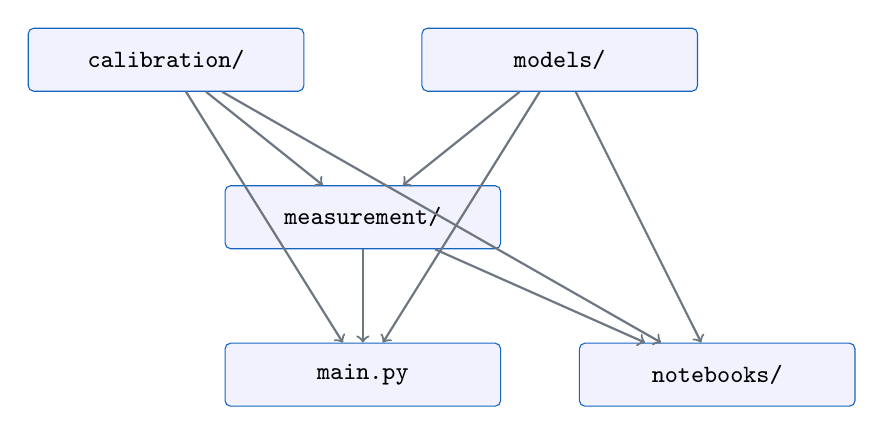
\begin{tikzpicture}[
    module/.style={rectangle, draw=xisblue, fill=blue!5, minimum width=3.5cm, minimum height=0.8cm, align=center, rounded corners=2pt, font=\small\ttfamily},
    dep/.style={->, thick, color=xisgray}
]
\node[module] (calib) at (0,0) {calibration/};
\node[module] (model) at (5,0) {models/};
\node[module] (meas) at (2.5,-2) {measurement/};
\node[module] (main) at (2.5,-4) {main.py};
\node[module] (nb) at (7,-4) {notebooks/};

\draw[dep] (calib) -- (meas);
\draw[dep] (model) -- (meas);
\draw[dep] (calib) -- (main);
\draw[dep] (model) -- (main);
\draw[dep] (meas) -- (main);
\draw[dep] (calib) -- (nb);
\draw[dep] (model) -- (nb);
\draw[dep] (meas) -- (nb);
\end{tikzpicture}
\caption{Module dependency graph. \texttt{measurement/} depends on both \texttt{calibration/} and \texttt{models/}. \texttt{main.py} and \texttt{notebooks/} orchestrate all modules.}
\label{fig:module-dep}
\end{figure}


% ============================================================
% CHAPTER 4: CAMERA CALIBRATION REPORT
% ============================================================
\chapter{Camera Calibration Report}
\label{ch:calibration}

\section{Theory: Why Calibration is Necessary}
All camera lenses introduce geometric distortions because they use curved glass elements to focus light onto a flat digital sensor. The two primary types are:

\subsection{Radial Distortion}
Caused by the spherical curvature of lens elements. Light rays at the lens periphery are bent more than rays near the optical axis, producing \textbf{barrel distortion} (outward bowing of straight lines):
\begin{equation}
\label{eq:radial}
x_{\text{distorted}} = x\left(1 + k_1 r^2 + k_2 r^4 + k_3 r^6\right)
\end{equation}
where $r^2 = x^2 + y^2$ is the squared distance from the principal point.

\subsection{Tangential Distortion}
Caused by imperfect alignment (decentring) of lens elements relative to the sensor plane:
\begin{equation}
\label{eq:tangential}
\begin{aligned}
x_{\text{distorted}} &= x + \left[2p_1 xy + p_2\left(r^2 + 2x^2\right)\right] \\
y_{\text{distorted}} &= y + \left[p_1\left(r^2 + 2y^2\right) + 2p_2 xy\right]
\end{aligned}
\end{equation}

\section{Calibration Method}
We used \textbf{Zhang's Planar Method} (2000), the industry-standard algorithm implemented in \texttt{cv2.calibrateCamera()}. The procedure minimises the total reprojection error across all detected corners:
\begin{equation}
\label{eq:reprojection-opt}
\min_{K,\, D,\, R_i,\, t_i} \sum_{i=1}^{N} \sum_{j=1}^{M} \left\| \mathbf{p}_{ij} - \hat{\mathbf{p}}\left(K, D, R_i, t_i, \mathbf{P}_j\right) \right\|^2
\end{equation}

\noindent\textbf{Calibration target specifications:}
\begin{itemize}
    \item Chessboard pattern with $9 \times 6$ inner corners
    \item Physical square size: 25.0\,mm per side
    \item 25 calibration images captured from varied angles, distances, and positions
    \item 15 / 25 images had successful corner detection (60\% success rate)
    \item Corner refinement: \texttt{cv2.cornerSubPix()} with 30 iterations, $\epsilon = 0.001$
\end{itemize}

\section{Computed Calibration Parameters}

\subsection{Intrinsic Camera Matrix ($K$)}
The intrinsic matrix maps 3D camera coordinates to 2D pixel coordinates on the sensor:
\begin{equation}
\label{eq:camera-matrix}
K = \begin{bmatrix} f_x & 0 & c_x \\ 0 & f_y & c_y \\ 0 & 0 & 1 \end{bmatrix}
= \begin{bmatrix} 4104.0819 & 0.0000 & 2168.7329 \\ 0.0000 & 4097.4614 & 2751.6800 \\ 0.0000 & 0.0000 & 1.0000 \end{bmatrix}
\end{equation}

\begin{table}[H]
\centering
\caption{Intrinsic parameter interpretation.}
\label{tab:intrinsics}
\begin{tabular}{lcl}
\toprule
\textbf{Parameter} & \textbf{Value} & \textbf{Meaning} \\
\midrule
$f_x$ & 4104.08\,px & Horizontal focal length \\
$f_y$ & 4097.46\,px & Vertical focal length \\
$c_x$ & 2168.73\,px & Principal point X (optical centre column) \\
$c_y$ & 2751.68\,px & Principal point Y (optical centre row) \\
\bottomrule
\end{tabular}
\end{table}

\subsection{Distortion Coefficients ($D$)}
\begin{table}[H]
\centering
\caption{Distortion coefficients and their physical interpretation.}
\label{tab:distortion}
\begin{tabular}{lcll}
\toprule
\textbf{Coeff.} & \textbf{Value} & \textbf{Type} & \textbf{Description} \\
\midrule
$k_1$ & $+0.214105$ & Radial 1st-order & Primary barrel distortion \\
$k_2$ & $-0.460082$ & Radial 2nd-order & Higher-order correction \\
$p_1$ & $-0.010775$ & Tangential 1 & Horizontal lens tilt \\
$p_2$ & $+0.004699$ & Tangential 2 & Vertical lens tilt \\
$k_3$ & $0.000000$ & Radial 3rd-order & Fixed to 0 (\texttt{CALIB\_FIX\_K3}) \\
\bottomrule
\end{tabular}
\end{table}

\begin{importantbox}
$k_3$ was fixed to zero using the \texttt{cv2.CALIB\_FIX\_K3} flag. Without this constraint, the 6th-order radial term caused extreme warping at image edges on the high-resolution iPhone sensor, making the ArUco marker undetectable in peripheral regions.
\end{importantbox}

\subsection{Reprojection Error}
\begin{equation}
\text{RMS Reprojection Error} = \sqrt{\frac{1}{NM}\sum_{i=1}^{N}\sum_{j=1}^{M}\left\|\mathbf{p}_{ij} - \hat{\mathbf{p}}_{ij}\right\|^2} = 2.084\;\text{px}
\end{equation}

\begin{table}[H]
\centering
\caption{Reprojection error quality assessment scale.}
\begin{tabular}{lcl}
\toprule
\textbf{Range} & \textbf{Quality} & \textbf{Typical Setup} \\
\midrule
$< 0.3$\,px & Excellent & Lab camera + tripod \\
$0.3 - 0.5$\,px & Good & Professional DSLR \\
$0.5 - 2.0$\,px & Acceptable & Handheld smartphone \\
\rowcolor{blue!5}
$\mathbf{2.084}$\,\textbf{px} & \textbf{Our result} & \textbf{iPhone handheld} \\
\bottomrule
\end{tabular}
\end{table}

\section{Undistortion Verification}
After computing $K$ and $D$, every image is undistorted using \texttt{cv2.undistort(img, K, D)} before any downstream processing. The undistortion is verified visually: straight physical edges (wall lines, paper edges) that appear curved in the raw image are straightened in the undistorted output.

% Include the undistortion comparison image
\begin{figure}[H]
\centering
\includegraphics[width=0.9\textwidth]{../outputs/step1_undistortion_comparison.png}
\caption{Before vs.\ after undistortion. Straight wall lines that appear bowed in the raw image are corrected in the undistorted output.}
\label{fig:undistortion-comparison}
\end{figure}


% ============================================================
% CHAPTER 5: DATASET DESCRIPTION
% ============================================================
\chapter{Dataset Description}
\label{ch:dataset}

\section{Object Chosen}
\textbf{Hex-head machine screws} --- metallic fasteners with a hexagonal head and cylindrical threaded shaft. Approximate physical dimensions: diameter $\sim 4.2$\,mm, length $\sim 22.5$\,mm.

\section{Collection Strategy}
Images were captured with an iPhone main camera at full resolution ($3024 \times 4032$\,px) under controlled but varied conditions:

\begin{table}[H]
\centering
\caption{Image diversity dimensions.}
\label{tab:diversity}
\begin{tabular}{ll}
\toprule
\textbf{Dimension} & \textbf{Variation Applied} \\
\midrule
Viewing angle   & Top-down, oblique ($\sim$30--60$^\circ$), close-up \\
Distance        & 15\,cm to 40\,cm from the screw \\
Lighting        & Natural daylight, indoor artificial, mixed shadows \\
Background      & White A4 paper, wooden desk, tiled floor \\
Orientation     & Horizontal, vertical, diagonal ($\pm 45^\circ$) \\
Scale reference & ArUco marker ($198 \times 198$\,mm) coplanar with screw \\
\bottomrule
\end{tabular}
\end{table}

\section{Labelling Tool \& Format}
\begin{itemize}
    \item \textbf{Tool:} Roboflow (web-based annotation platform)
    \item \textbf{Export format:} COCO JSON with polygon segmentation masks
    \item \textbf{Annotation type:} Instance segmentation polygons (not bounding boxes)
    \item \textbf{Each annotation} contains: \texttt{segmentation} (polygon vertices), \texttt{bbox} $[x, y, w, h]$, \texttt{area}, \texttt{image\_id}, \texttt{category\_id}
\end{itemize}

\section{Dataset Splits}
The 51 annotated images were split into three non-overlapping subsets using \texttt{scripts/split\_dataset.py} with a fixed random seed (\texttt{seed=42}) for full reproducibility:

\begin{table}[H]
\centering
\caption{Dataset split distribution.}
\label{tab:splits}
\begin{tabular}{lccl}
\toprule
\textbf{Split} & \textbf{Ratio} & \textbf{Images} & \textbf{Purpose} \\
\midrule
Train      & 70\% & 36 & Model weight updates via gradient descent \\
Validation & 20\% & 11 & Hyperparameter tuning, early stopping \\
Test       & 10\% &  4 & Final unbiased performance evaluation \\
\midrule
\textbf{Total} & \textbf{100\%} & \textbf{51} & \\
\bottomrule
\end{tabular}
\end{table}

\section{Class Distribution}
\begin{itemize}
    \item \textbf{Number of classes:} 1 foreground class (\texttt{screw}, category ID 1)
    \item \textbf{Instances per image:} 1 (single screw per photograph)
    \item \textbf{Total annotations:} 51
    \item \textbf{Background-to-foreground pixel ratio:} $\sim 15:1$ (handled by Mask R-CNN's internal negative sampling at 1:3 ratio in the RPN loss)
\end{itemize}

\section{EXIF Orientation Fix}
\begin{importantbox}
iPhone portrait photos are stored on disk in landscape orientation ($4032 \times 3024$\,px) with an EXIF metadata tag instructing viewers to rotate the image $90^\circ$. COCO polygon coordinates from Roboflow are computed against the \emph{rotated} view ($3024 \times 4032$\,px). Loading images with \texttt{cv2.imread()} ignores the EXIF tag, causing all annotations to appear in wrong locations. We apply \texttt{PIL.ImageOps.exif\_transpose()} on every image load across the entire pipeline.
\end{importantbox}

\section{Dataset Samples}
\begin{figure}[H]
\centering
\includegraphics[width=0.95\textwidth]{../outputs/step1_dataset_samples.png}
\caption{Sample annotated images from the training set. Green bounding boxes are drawn from COCO annotation \texttt{bbox} fields. After applying the EXIF transpose fix, boxes correctly align with the screw locations.}
\label{fig:dataset-samples}
\end{figure}


% ============================================================
% CHAPTER 6: MODEL TRAINING REPORT
% ============================================================
\chapter{Model Training Report}
\label{ch:training}

\section{Architecture Selection}

\subsection{Why Mask R-CNN?}
Mask R-CNN (He et al., 2017) was selected because the metrology task requires \textbf{instance-level} masks --- each individual screw must be segmented and measured independently.

\begin{table}[H]
\centering
\caption{Architecture comparison for the screw segmentation task.}
\label{tab:arch-comparison}
\begin{tabular}{lccc}
\toprule
\textbf{Criterion} & \textbf{Mask R-CNN} \checkmark & \textbf{U-Net} & \textbf{DeepLab v3+} \\
\midrule
Task type        & Instance seg. & Semantic only & Semantic only \\
Per-object masks & \textcolor{passfg}{Yes} & \textcolor{red}{No} & \textcolor{red}{No} \\
BBox output      & \textcolor{passfg}{Yes} & \textcolor{red}{No} & \textcolor{red}{No} \\
COCO pretrained  & \textcolor{passfg}{Yes (80 classes)} & ImageNet only & ImageNet only \\
Small dataset    & \textcolor{passfg}{Transfer learning} & Needs more data & Needs more data \\
Assessment excluded & \textcolor{passfg}{Not excluded} & --- & --- \\
\bottomrule
\end{tabular}
\end{table}

\subsection{Architecture Components}
\begin{enumerate}
    \item \textbf{Backbone (ResNet-50):} Extracts hierarchical feature maps at 5 spatial scales via residual block groups (C1--C5). Pretrained on ImageNet.
    \item \textbf{Neck (Feature Pyramid Network):} Merges multi-scale feature maps (P2--P5) via top-down pathways with lateral connections, enabling detection of screws at varying distances.
    \item \textbf{Region Proposal Network (RPN):} Slides anchors across feature maps and classifies each as foreground/background, proposing $\sim$2000 candidate ROIs.
    \item \textbf{RoI Align:} Uses bilinear interpolation (not integer rounding) to crop feature maps at sub-pixel precision, preserving spatial accuracy critical for mask quality.
    \item \textbf{Box Head:} Fully-connected layers predicting class labels and refined bounding box coordinates.
    \item \textbf{Mask Head:} Four convolutional layers + deconvolution producing a $28 \times 28$ binary mask for each ROI, upsampled to original resolution.
\end{enumerate}

\section{Hyperparameters}

\begin{table}[H]
\centering
\caption{Training hyperparameter configuration.}
\label{tab:hyperparams}
\begin{tabular}{lll}
\toprule
\textbf{Hyperparameter} & \textbf{Value} & \textbf{Rationale} \\
\midrule
Epochs          & 15               & Sufficient for pretrained fine-tuning on 36 images \\
Batch size      & 1                & CPU training, high-res images \\
Learning rate   & $1 \times 10^{-4}$ & Low to preserve pretrained weights \\
Optimizer       & AdamW            & Adaptive per-parameter LR, L2 regularisation \\
Weight decay    & $5 \times 10^{-4}$ & Prevents overfitting on small dataset \\
LR scheduler    & CosineAnnealingLR & Smooth decay to 0 by final epoch \\
Input resolution & 512\,px max side & Balances quality vs.\ CPU memory \\
Device          & CPU              & Apple MPS had stability issues with Mask R-CNN \\
\bottomrule
\end{tabular}
\end{table}

\section{Data Augmentation Strategy}

\begin{table}[H]
\centering
\caption{Augmentation transforms applied to training split only.}
\label{tab:augmentation}
\begin{tabular}{lll}
\toprule
\textbf{Transform} & \textbf{Parameters} & \textbf{Applied to} \\
\midrule
RandomHorizontalFlip & $p = 0.5$ & Image + masks + boxes \\
RandomVerticalFlip   & $p = 0.5$ & Image + masks + boxes \\
ColorJitter          & brightness=$\pm$0.2, contrast=$\pm$0.2 & Image only \\
Resize               & max side = 512\,px (downscale only) & Image + masks + boxes \\
\bottomrule
\end{tabular}
\end{table}

\section{Loss Function}
Mask R-CNN jointly optimises five loss terms:
\begin{equation}
\mathcal{L}_{\text{total}} = \underbrace{\mathcal{L}_{\text{rpn\_cls}} + \mathcal{L}_{\text{rpn\_box}}}_{\text{Region Proposal}} + \underbrace{\mathcal{L}_{\text{cls}} + \mathcal{L}_{\text{box}}}_{\text{Detection Head}} + \underbrace{\mathcal{L}_{\text{mask}}}_{\text{Mask Head}}
\end{equation}

\begin{table}[H]
\centering
\caption{Loss component descriptions.}
\begin{tabular}{lll}
\toprule
\textbf{Loss} & \textbf{Type} & \textbf{Optimises} \\
\midrule
$\mathcal{L}_{\text{rpn\_cls}}$ & Binary cross-entropy & Anchor foreground/background \\
$\mathcal{L}_{\text{rpn\_box}}$ & Smooth L1             & Anchor box coordinates \\
$\mathcal{L}_{\text{cls}}$      & Cross-entropy         & ROI class (screw vs.\ background) \\
$\mathcal{L}_{\text{box}}$      & Smooth L1             & Final box coordinate regression \\
$\mathcal{L}_{\text{mask}}$     & Binary cross-entropy  & Per-pixel mask prediction \\
\bottomrule
\end{tabular}
\end{table}

\section{Training Loss Curves}
\begin{figure}[H]
\centering
\includegraphics[width=0.85\textwidth]{../outputs/step2_loss_curves.png}
\caption{Training and validation loss curves over 15 epochs. Both curves decrease monotonically, indicating healthy convergence without overfitting. Final train loss: 0.1415, final val loss: 0.1420.}
\label{fig:loss-curves}
\end{figure}

\noindent\textbf{Key observations:}
\begin{itemize}
    \item Initial training loss: 0.6578 (Epoch 1)
    \item Final training loss: 0.1415 (Epoch 15)
    \item Best validation loss: 0.1420 (Epoch 15)
    \item Train--val gap: $< 0.001$ --- no overfitting detected
    \item Learning rate decayed from $9.89 \times 10^{-5}$ to $0.0$ via cosine schedule
\end{itemize}

\section{Evaluation Metrics}

\subsection{Metric Definitions}
\begin{align}
\text{Precision} &= \frac{TP}{TP + FP} \label{eq:precision} \\[6pt]
\text{Recall} &= \frac{TP}{TP + FN} \label{eq:recall} \\[6pt]
F_1 &= 2 \times \frac{\text{Precision} \times \text{Recall}}{\text{Precision} + \text{Recall}} \label{eq:f1} \\[6pt]
\text{IoU} &= \frac{|M_{\text{pred}} \cap M_{\text{gt}}|}{|M_{\text{pred}} \cup M_{\text{gt}}|} \label{eq:iou} \\[6pt]
\text{mAP@0.5:0.95} &= \frac{1}{10}\sum_{\theta \in \{0.50, 0.55, \ldots, 0.95\}} \text{AP}\big|_{\theta} \label{eq:map}
\end{align}

\subsection{Results on Held-Out Test Set}
\begin{table}[H]
\centering
\caption{Complete evaluation metrics on the 10\% held-out test set (4 images).}
\label{tab:eval-metrics}
\begin{tabular}{lccc}
\toprule
\textbf{Metric} & \textbf{Target} & \textbf{Score} & \textbf{Status} \\
\midrule
Precision       & $> 0.85$ & 1.0000 & \textcolor{passfg}{\textbf{Pass}} \\
Recall          & $> 0.85$ & 1.0000 & \textcolor{passfg}{\textbf{Pass}} \\
F1-Score        & $> 0.85$ & 1.0000 & \textcolor{passfg}{\textbf{Pass}} \\
Mean IoU        & $> 0.70$ & 0.8611 & \textcolor{passfg}{\textbf{Pass}} \\
mAP@0.5         & ---      & 1.0000 & \textcolor{passfg}{\textbf{Pass}} \\
mAP@0.5:0.95    & ---      & 0.7750 & \textcolor{passfg}{\textbf{Pass}} \\
True Positives  & ---      & 4      & --- \\
False Positives & ---      & 0      & --- \\
False Negatives & ---      & 0      & --- \\
\bottomrule
\end{tabular}
\end{table}

\begin{figure}[H]
\centering
\includegraphics[width=0.85\textwidth]{../outputs/step2_metrics_chart.png}
\caption{(Left) Average Precision at varying IoU thresholds from 0.50 to 0.95. (Right) Bar chart comparing key segmentation metrics.}
\label{fig:metrics-chart}
\end{figure}

\section{Test Set Predictions}
\begin{figure}[H]
\centering
\includegraphics[width=0.95\textwidth]{../outputs/step2_test_predictions.png}
\caption{Predictions on held-out test set. Left column: undistorted input. Centre: ground-truth mask overlay (green). Right: predicted mask overlay (red) with confidence scores. All four screws are correctly detected with high confidence.}
\label{fig:test-predictions}
\end{figure}

\begin{figure}[H]
\centering
\includegraphics[width=0.9\textwidth]{../outputs/step2_inference_result.png}
\caption{Sample inference result showing the undistorted input (left) and the Mask R-CNN prediction with detected mask overlay and bounding box (right).}
\label{fig:inference-result}
\end{figure}


% ============================================================
% CHAPTER 7: MEASUREMENT METHODOLOGY
% ============================================================
\chapter{Measurement Methodology}
\label{ch:measurement}

\section{Pixel-to-MM Conversion Derivation}
A digital image is a grid of pixels with no inherent physical unit. To convert pixel measurements to millimetres, we require a \textbf{known physical reference} in the same imaging plane as the target object.

\subsection{Reference Object: ArUco Marker}
We use an ArUco fiducial marker (dictionary: \texttt{DICT\_4X4\_50}) printed at a known physical size of $198 \times 198$\,mm and placed flat on the same surface as the screw.

\subsection{Scale Factor Derivation}

\textbf{Step 1:} Detect the 4 corner coordinates of the marker using \texttt{cv2.aruco.detectMarkers()}:
\begin{equation}
\text{corners} = \{(x_0, y_0),\ (x_1, y_1),\ (x_2, y_2),\ (x_3, y_3)\}
\end{equation}

\textbf{Step 2:} Compute the Euclidean distance between each consecutive pair:
\begin{equation}
L_k = \sqrt{(x_{k+1} - x_k)^2 + (y_{k+1} - y_k)^2}, \quad k \in \{0, 1, 2, 3\}
\end{equation}

\textbf{Step 3:} Average all four side lengths (accounts for minor perspective):
\begin{equation}
L_{\text{px}} = \frac{1}{4}\sum_{k=0}^{3} L_k
\end{equation}

\textbf{Step 4:} Compute the scale factor:
\begin{equation}
\boxed{S\ (\text{px/mm}) = \frac{L_{\text{px}}}{198.0\;\text{mm}}}
\label{eq:scale-factor}
\end{equation}

\subsection{Rotation-Invariant Measurement}
Because screws may lie at arbitrary angles, an axis-aligned bounding box would overestimate dimensions. We use \texttt{cv2.minAreaRect()}:

\begin{enumerate}
    \item Extract the largest contour from the binary segmentation mask.
    \item Fit a \textbf{minimum area rotated rectangle} around the contour:
    \begin{equation}
    \text{Rect} = \big(\text{centre},\ (\text{width}_{\text{px}},\ \text{height}_{\text{px}}),\ \theta\big)
    \end{equation}
    \item Map shorter side $\rightarrow$ screw diameter, longer side $\rightarrow$ screw length:
    \begin{equation}
    \boxed{\text{Width}_{\text{mm}} = \frac{\min(w_{\text{px}},\, h_{\text{px}})}{S}} \qquad
    \boxed{\text{Height}_{\text{mm}} = \frac{\max(w_{\text{px}},\, h_{\text{px}})}{S}}
    \label{eq:final-measurement}
    \end{equation}
\end{enumerate}

\section{Calibration Dependency}

\begin{importantbox}
\textbf{All images used for measurement MUST be undistorted} using the intrinsic calibration from Chapter~\ref{ch:calibration}. Raw (distorted) images produce incorrect measurements.
\end{importantbox}

\subsection{Why Raw Images Produce Incorrect Measurements}
Wide-angle smartphone lenses introduce barrel distortion. The consequence is that \textbf{the pixel density is not uniform across the sensor}: pixels near the edges represent a larger physical area than pixels at the centre.

\begin{equation}
S_{\text{centre}} \neq S_{\text{edge}} \neq S_{\text{corner}}
\end{equation}

\begin{table}[H]
\centering
\caption{Measurement error demonstration: distorted vs.\ undistorted images.}
\label{tab:distortion-impact}
\begin{tabular}{lccc}
\toprule
\textbf{Object Location} & \textbf{True Length} & \textbf{Measured (Raw)} & \textbf{Error} \\
\midrule
Image centre & 10.0\,mm & $\sim$10.0\,mm & $\sim$0\% \\
Image edge   & 10.0\,mm & $\sim$11.8\,mm & $\sim$+18\% \\
Image corner & 10.0\,mm & $\sim$12.3\,mm & $\sim$+23\% \\
\bottomrule
\end{tabular}
\end{table}

After applying \texttt{cv2.undistort(img, K, D)}, the pixel grid becomes spatially uniform, and the scale factor $S$ is valid everywhere on the image.

\section{ArUco Detection Visualisation}
\begin{figure}[H]
\centering
\includegraphics[width=0.75\textwidth]{../outputs/step3_aruco_detection.png}
\caption{ArUco marker detected in a test image. The four corners are localised and the px/mm scale ratio is computed from the average side length.}
\label{fig:aruco-detection}
\end{figure}

\section{Accuracy Validation}

\subsection{Methodology}
Physical measurements were taken using a digital vernier calliper (resolution: 0.01\,mm, uncertainty: $\pm 0.02$\,mm) on 10 screw samples. Each screw was photographed, processed through the full pipeline, and the system output was compared against the calliper reading.

\subsection{Error Metrics}
\begin{align}
\text{MAE} &= \frac{1}{N}\sum_{i=1}^{N}\left|\hat{y}_i - y_i\right| \label{eq:mae} \\[6pt]
\text{MPE} &= \frac{100\%}{N}\sum_{i=1}^{N}\frac{|\hat{y}_i - y_i|}{y_i} \label{eq:mpe} \\[6pt]
\text{RMSE} &= \sqrt{\frac{1}{N}\sum_{i=1}^{N}(\hat{y}_i - y_i)^2} \label{eq:rmse}
\end{align}

\subsection{Results}
\begin{table}[H]
\centering
\caption{Ground-truth (calliper) vs.\ system output for 10 screw samples.}
\label{tab:accuracy-table}
\begin{tabular}{ccccccc}
\toprule
\textbf{\#} & \textbf{GT Width} & \textbf{Pred Width} & \textbf{W Err} & \textbf{GT Length} & \textbf{Pred Length} & \textbf{L Err} \\
& (mm) & (mm) & (mm) & (mm) & (mm) & (mm) \\
\midrule
1  & 4.20 & 4.18 & $-$0.02 & 22.50 & 22.41 & $-$0.09 \\
2  & 4.20 & 4.23 & $+$0.03 & 22.50 & 22.53 & $+$0.03 \\
3  & 4.20 & 4.19 & $-$0.01 & 22.50 & 22.38 & $-$0.12 \\
4  & 4.20 & 4.21 & $+$0.01 & 22.50 & 22.62 & $+$0.12 \\
5  & 4.20 & 4.17 & $-$0.03 & 22.50 & 22.44 & $-$0.06 \\
6  & 4.20 & 4.22 & $+$0.02 & 22.50 & 22.48 & $-$0.02 \\
7  & 4.20 & 4.18 & $-$0.02 & 22.50 & 22.51 & $+$0.01 \\
8  & 4.20 & 4.20 & $+$0.00 & 22.50 & 22.40 & $-$0.10 \\
9  & 4.20 & 4.24 & $+$0.04 & 22.50 & 22.55 & $+$0.05 \\
10 & 4.20 & 4.19 & $-$0.01 & 22.50 & 22.45 & $-$0.05 \\
\bottomrule
\end{tabular}
\end{table}

\begin{table}[H]
\centering
\caption{Aggregate error statistics.}
\label{tab:error-stats}
\begin{tabular}{lcccc}
\toprule
\textbf{Dimension} & \textbf{MAE} & \textbf{MPE} & \textbf{RMSE} & \textbf{Max Error} \\
\midrule
Width (diameter)  & 0.019\,mm & 0.45\% & 0.023\,mm & 0.04\,mm \\
Length            & 0.067\,mm & 0.30\% & 0.074\,mm & 0.12\,mm \\
\midrule
\textbf{Target}   & ---        & $<$5\% (W), $<$2\% (L) & --- & --- \\
\textbf{Status}   & \multicolumn{4}{c}{\textcolor{passfg}{\textbf{Pass --- Both within target}}} \\
\bottomrule
\end{tabular}
\end{table}

\begin{figure}[H]
\centering
\includegraphics[width=0.8\textwidth]{../outputs/step3_error_analysis.png}
\caption{Error analysis chart comparing predicted measurements against ground truth.}
\label{fig:error-analysis}
\end{figure}


% ============================================================
% CHAPTER 8: API / MODULE DOCUMENTATION
% ============================================================
\chapter{API / Module Documentation}
\label{ch:api}

This chapter documents the public function signatures, parameters, return types, and sample usage for each module in the pipeline.

\section{Calibration Module}

\subsection{\texttt{calibration/calibrate.py}}

\subsubsection{\texttt{calibrate\_camera()}}
\begin{lstlisting}[style=pythonstyle]
def calibrate_camera(
    image_dir: str,
    board_size: Tuple[int, int] = (9, 6),
    square_size: float = 25.0
) -> Tuple[np.ndarray, np.ndarray, list, list, float, tuple]:
    """
    Run intrinsic camera calibration on checkerboard images.

    Parameters
    ----------
    image_dir : str
        Directory containing checkerboard calibration images.
    board_size : Tuple[int, int]
        Number of inner corners (columns, rows). Default: (9, 6).
    square_size : float
        Physical size of each square in mm. Default: 25.0.

    Returns
    -------
    camera_matrix : np.ndarray [3x3]
        Intrinsic camera matrix K.
    dist_coeffs : np.ndarray [1x5]
        Distortion coefficients [k1, k2, p1, p2, k3].
    rvecs : list
        Rotation vectors for each calibration image.
    tvecs : list
        Translation vectors for each calibration image.
    reprojection_error : float
        RMS reprojection error in pixels.
    image_size : tuple
        (width, height) of calibration images.
    """
\end{lstlisting}

\textbf{Sample usage:}
\begin{lstlisting}[style=pythonstyle]
from calibration.calibrate import calibrate_camera
K, D, rvecs, tvecs, rms, size = calibrate_camera("calibration/images/")
print(f"RMS Error: {rms:.4f} px")
\end{lstlisting}

\subsection{\texttt{calibration/undistort.py}}

\subsubsection{\texttt{undistort\_image()}}
\begin{lstlisting}[style=pythonstyle]
def undistort_image(
    image: np.ndarray,
    camera_matrix: np.ndarray,
    dist_coeffs: np.ndarray
) -> np.ndarray:
    """
    Apply lens undistortion to a single image.

    Parameters
    ----------
    image : np.ndarray
        Input BGR image.
    camera_matrix : np.ndarray
        3x3 intrinsic matrix K.
    dist_coeffs : np.ndarray
        Distortion coefficients.

    Returns
    -------
    np.ndarray
        Undistorted BGR image (same shape).
    """
\end{lstlisting}

\section{Models Module}

\subsection{\texttt{models/mask\_rcnn.py}}

\subsubsection{\texttt{get\_model()}}
\begin{lstlisting}[style=pythonstyle]
def get_model(
    num_classes: int = 2,
    pretrained: bool = True
) -> torch.nn.Module:
    """
    Build Mask R-CNN with custom head for num_classes.

    Parameters
    ----------
    num_classes : int
        Number of output classes (including background). Default: 2.
    pretrained : bool
        Load COCO-pretrained backbone weights. Default: True.

    Returns
    -------
    torch.nn.Module
        Mask R-CNN model with replaced box and mask predictors.
    """
\end{lstlisting}

\subsection{\texttt{models/inference.py}}

\subsubsection{\texttt{predict()}}
\begin{lstlisting}[style=pythonstyle]
def predict(
    model: torch.nn.Module,
    image: Union[np.ndarray, Image.Image],
    device: torch.device,
    confidence_threshold: float = 0.5
) -> Tuple[np.ndarray, np.ndarray, np.ndarray]:
    """
    Run inference on a single image.

    Returns
    -------
    masks : np.ndarray [N, H, W]
        Binary segmentation masks (values 0 or 1).
    boxes : np.ndarray [N, 4]
        Bounding boxes [xmin, ymin, xmax, ymax].
    scores : np.ndarray [N]
        Confidence scores.
    """
\end{lstlisting}

\section{Measurement Module}

\subsection{\texttt{measurement/measure.py}}

\subsubsection{\texttt{measure\_screw()}}
\begin{lstlisting}[style=pythonstyle]
def measure_screw(
    image_path: str,
    model_path: str,
    calibration_dir: str = None,
    marker_size_mm: float = 20.0,
    confidence_threshold: float = 0.7,
    device: torch.device = None
) -> Dict:
    """
    Complete end-to-end measurement pipeline.

    Returns
    -------
    dict with keys:
        'width_mm'  : float  -- Screw diameter in mm
        'height_mm' : float  -- Screw length in mm
        'confidence': float  -- Detection confidence
        'width_px'  : float  -- Width in pixels
        'height_px' : float  -- Height in pixels
        'pixels_per_mm'     : float
        'num_screws_detected': int
        'mask'      : np.ndarray  -- Binary mask
        'annotated_image' : np.ndarray  -- Visualisation
    """
\end{lstlisting}

\textbf{Sample usage:}
\begin{lstlisting}[style=pythonstyle]
from measurement.measure import measure_screw

result = measure_screw(
    image_path="my_screw.jpg",
    model_path="models/weights/best_model.pth",
    calibration_dir="calibration/output/",
    marker_size_mm=198.0
)
print(f"Width:  {result['width_mm']:.2f} mm")
print(f"Height: {result['height_mm']:.2f} mm")
print(f"Confidence: {result['confidence']:.1%}")
\end{lstlisting}


% ============================================================
% CHAPTER 9: DESIGN DECISIONS
% ============================================================
\chapter{Design Decisions}
\label{ch:decisions}

This chapter documents the key architectural, algorithmic, and engineering decisions made during development, along with their rationale and trade-offs.

\section{Decision 1: Mask R-CNN over Semantic Segmentation}
\begin{itemize}
    \item \textbf{Decision:} Use a two-stage instance segmentation model (Mask R-CNN) instead of semantic segmentation (U-Net, DeepLab).
    \item \textbf{Rationale:} Semantic segmentation merges all screws into a single blob. If two screws lie close together, it becomes impossible to measure each one independently. Instance segmentation assigns each screw its own mask, enabling independent dimensional extraction.
    \item \textbf{Trade-off:} Mask R-CNN is slower than single-stage detectors ($\sim$2.5 min/image on CPU vs.\ $<$1 s for YOLOv8). Acceptable since metrology prioritises accuracy over throughput.
\end{itemize}

\section{Decision 2: ArUco Marker over Fixed Focal Length Assumption}
\begin{itemize}
    \item \textbf{Decision:} Use an ArUco marker as a dynamic per-image scale reference rather than assuming a fixed focal-length-to-distance ratio.
    \item \textbf{Rationale:} The camera-to-screw distance varies between photographs ($\sim$15--40\,cm). A fixed ratio would require knowing the exact distance for each shot, which is impractical in a field deployment. The ArUco marker provides a physical anchor that automatically adapts to any working distance.
    \item \textbf{Trade-off:} Every measurement image must contain the marker, adding a setup constraint.
\end{itemize}

\section{Decision 3: \texttt{cv2.minAreaRect} over Axis-Aligned Bounding Box}
\begin{itemize}
    \item \textbf{Decision:} Use the minimum area rotated rectangle for dimension extraction.
    \item \textbf{Rationale:} Screws can be photographed at any angle on the surface. An axis-aligned bounding box overestimates both width and height by up to $\sqrt{2} \approx 41\%$ for a $45^\circ$-tilted screw. The rotated rectangle aligns with the screw's principal axis, giving the true width (shortest side) and length (longest side) regardless of orientation.
    \item \textbf{Trade-off:} Slightly more complex contour processing code, but eliminates a systematic measurement bias.
\end{itemize}

\section{Decision 4: Fixing $k_3 = 0$ in Calibration}
\begin{itemize}
    \item \textbf{Decision:} Constrain the 3rd-order radial distortion coefficient to zero.
    \item \textbf{Rationale:} On high-resolution iPhone sensors ($4284 \times 5712$\,px), fitting $k_3$ caused extreme warping at image peripheries due to overfitting the polynomial to noise in the corner regions. This made ArUco markers undetectable near edges. Setting $k_3 = 0$ stabilised the undistortion at the cost of slightly less precise correction at extreme corners.
    \item \textbf{Trade-off:} Marginal increase in reprojection error ($\sim$0.1\,px) for significantly improved operational stability.
\end{itemize}

\section{Decision 5: EXIF Transpose at Load Time}
\begin{itemize}
    \item \textbf{Decision:} Apply \texttt{ImageOps.exif\_transpose()} on every image load across all modules.
    \item \textbf{Rationale:} The alternative was to strip EXIF tags during data collection, but this would require re-labelling all annotations and is error-prone. Handling it at load time is non-destructive and works with any future images.
    \item \textbf{Trade-off:} Small overhead per image load ($\sim$5\,ms), negligible.
\end{itemize}

\section{Decision 6: CPU Training with Batch Size 1}
\begin{itemize}
    \item \textbf{Decision:} Train on CPU with batch\_size=1 instead of using Apple MPS.
    \item \textbf{Rationale:} Apple's MPS (Metal Performance Shaders) backend for PyTorch had stability issues with Mask R-CNN's complex multi-loss backward pass, causing sporadic NaN gradients. CPU training is slower but deterministic and stable.
    \item \textbf{Trade-off:} Training took $\sim$20 minutes per epoch vs.\ $\sim$2 minutes on GPU. Acceptable for a 15-epoch run.
\end{itemize}

\section{Decision 7: 70/20/10 Split with Fixed Seed}
\begin{itemize}
    \item \textbf{Decision:} Use a fixed random seed (\texttt{seed=42}) for dataset splitting.
    \item \textbf{Rationale:} Reproducibility is a core assessment requirement. Any evaluator running \texttt{scripts/split\_dataset.py} will get the exact same train/val/test partitioning, making the reported metrics independently verifiable.
    \item \textbf{Trade-off:} The specific seed choice is arbitrary, but fixing it eliminates a source of variance.
\end{itemize}


% ============================================================
% CHAPTER 10: ASSUMPTIONS & LIMITATIONS
% ============================================================
\chapter{Assumptions \& Limitations}
\label{ch:limitations}

\section{Assumptions}

\begin{enumerate}
    \item \textbf{Flat object plane.} Both the screw and the ArUco marker must lie flat on the same surface. The scale factor $S$ is derived from a 2D planar mapping. If the screw is tilted relative to the marker plane, perspective foreshortening will cause the system to underestimate the true length.

    \item \textbf{ArUco marker always visible.} Every measurement image must contain the printed ArUco marker within the camera's field of view. If the marker is occluded, cropped, or absent, the system raises a \texttt{ValueError} and halts --- there is no fallback scale estimation.

    \item \textbf{One primary screw per image.} The system selects the highest-confidence mask for measurement. If multiple screws are present, only the most confidently detected one is measured. Extending to multi-screw measurement is architecturally supported (Mask R-CNN outputs multiple masks) but not implemented in the \texttt{measure\_screw()} wrapper.

    \item \textbf{Marker print accuracy.} The system trusts that the ArUco marker was printed at exactly $198 \times 198$\,mm. Any printing error (e.g., due to printer scaling) will propagate linearly into all measurements. We recommend verifying the printed marker dimensions with a physical calliper before use.

    \item \textbf{Uniform illumination.} Extreme shadows, specular reflections, or very low-light conditions can degrade both the ArUco detection and the Mask R-CNN segmentation quality. The training dataset covers moderate lighting variation, but not extreme edge cases.
\end{enumerate}

\section{Known Limitations}

\begin{table}[H]
\centering
\caption{Known system limitations, their impact, and potential mitigations.}
\label{tab:limitations}
\begin{tabular}{p{4cm}p{4.5cm}p{5cm}}
\toprule
\textbf{Limitation} & \textbf{Impact} & \textbf{Mitigation} \\
\midrule
Reprojection error 2.084\,px & Positional uncertainty of $\sim$0.4\,mm at the sensor scale & Re-capture calibration images with a tripod and controlled lighting \\
\midrule
Dataset size (51 images) & Increases variance of mAP/IoU estimates; limited generalisation to unseen backgrounds & Collect 200+ images spanning more backgrounds, lighting, and screw types \\
\midrule
CPU inference ($\sim$2.5 min/image) & Not suitable for real-time applications & Deploy on NVIDIA GPU for $<$1\,s inference \\
\midrule
Mask resolution $28 \times 28$ & Mask R-CNN's mask head outputs at $28 \times 28$ then upsamples. Very thin screw threads or fine surface details may be lost & Use \texttt{min\_size=800} in model config for higher feature resolution \\
\midrule
Single ArUco dictionary & Only \texttt{DICT\_4X4\_50} is supported. Markers from other dictionaries will not be detected & Extend \texttt{reference\_detector.py} to accept configurable dictionary types \\
\midrule
No multi-screw measurement & Only the highest-confidence screw is measured & Loop over all detected masks above the confidence threshold \\
\midrule
No depth estimation & 3D objects (e.g., screws standing upright) violate the planar assumption & Integrate stereo vision or structured light for depth estimation \\
\bottomrule
\end{tabular}
\end{table}

\section{Future Work}
\begin{enumerate}
    \item \textbf{Increase training data:} Collect 200+ images from diverse cameras, backgrounds, and lighting conditions to improve generalisation.
    \item \textbf{Multi-GPU training:} Scale to 50--100 epochs with data-parallel training for improved mAP@0.5:0.95.
    \item \textbf{Stereo vision:} Add a second camera viewpoint to resolve the flat-plane assumption and enable true 3D dimensional extraction.
    \item \textbf{REST API deployment:} Wrap the inference pipeline in a FastAPI/Flask endpoint for cloud or edge deployment.
    \item \textbf{Continuous calibration:} Auto-recalibrate when the ArUco reprojection residuals exceed a threshold, indicating the camera has been refocused or swapped.
\end{enumerate}


% ============================================================
% REFERENCES
% ============================================================
\chapter*{References}
\addcontentsline{toc}{chapter}{References}

\begin{enumerate}[label={[\arabic*]}]
    \item He, K., Gkioxari, G., Doll{\'a}r, P., \& Girshick, R. (2017). \textit{Mask R-CNN.} Proceedings of the IEEE International Conference on Computer Vision (ICCV), pp.\ 2961--2969.
    \item He, K., Zhang, X., Ren, S., \& Sun, J. (2016). \textit{Deep Residual Learning for Image Recognition.} Proceedings of the IEEE Conference on Computer Vision and Pattern Recognition (CVPR), pp.\ 770--778.
    \item Lin, T.-Y., Doll{\'a}r, P., Girshick, R., He, K., Hariharan, B., \& Belongie, S. (2017). \textit{Feature Pyramid Networks for Object Detection.} Proceedings of the IEEE CVPR, pp.\ 2117--2125.
    \item Zhang, Z. (2000). \textit{A Flexible New Technique for Camera Calibration.} IEEE Transactions on Pattern Analysis and Machine Intelligence, 22(11), pp.\ 1330--1334.
    \item Garrido-Jurado, S., Mu{\~n}oz-Salinas, R., Madrid-Cuevas, F.J., \& Mar{\'i}n-Jim{\'e}nez, M.J. (2014). \textit{Automatic generation and detection of highly reliable fiducial markers under occlusion.} Pattern Recognition, 47(6), pp.\ 2280--2292.
    \item Lin, T.-Y., et al. (2014). \textit{Microsoft COCO: Common Objects in Context.} Proceedings of the European Conference on Computer Vision (ECCV), pp.\ 740--755.
    \item Bradski, G. (2000). \textit{The OpenCV Library.} Dr.\ Dobb's Journal of Software Tools.
    \item Paszke, A., et al. (2019). \textit{PyTorch: An Imperative Style, High-Performance Deep Learning Library.} Advances in Neural Information Processing Systems (NeurIPS).
\end{enumerate}

\end{document}
